%%%%%%%%%%%%%%%%%%%%%%%%%%%%%%%%%%%%%
%                                   %
% Compile with XeLaTeX and biber    %
%                                   %
% Questions or comments:            %
%                                   %
% joshua dot mcneill at uga dot edu %
%                                   %
%%%%%%%%%%%%%%%%%%%%%%%%%%%%%%%%%%%%%

\documentclass{beamer}
  % Read in standard preamble (cosmetic stuff)
  %%%%%%%%%%%%%%%%%%%%%%%%%%%%%%%%%%%%%%%%%%%%%%%%%%%%%%%%%%%%%%%%
% This is a standard preamble used in for all slide documents. %
% It basically contains cosmetic settings.                     %
%                                                              %
% Joshua McNeill                                               %
% joshua dot mcneill at uga dot edu                            %
%%%%%%%%%%%%%%%%%%%%%%%%%%%%%%%%%%%%%%%%%%%%%%%%%%%%%%%%%%%%%%%%

% Beamer settings
% \usetheme{Berkeley}
\usetheme{CambridgeUS}
% \usecolortheme{dove}
% \usecolortheme{rose}
\usecolortheme{seagull}
\usefonttheme{professionalfonts}
\usefonttheme{serif}
\setbeamertemplate{bibliography item}{}

% Packages and settings
\usepackage{fontspec}
  \setmainfont{Charis SIL}
\usepackage{hyperref}
  \hypersetup{colorlinks=true,
              allcolors=blue}
\usepackage{graphicx}
  \graphicspath{{../../figures/}}
\usepackage[normalem]{ulem}
\usepackage{enumerate}

% Document information
\author{M. McNeill}
\title[FREN2001]{Français 2001}
\institute{\url{joshua.mcneill@uga.edu}}
\date{}

%% Custom commands
% Lexical items
\newcommand{\lexi}[1]{\textit{#1}}
% Gloss
\newcommand{\gloss}[1]{`#1'}
\newcommand{\tinygloss}[1]{{\tiny`#1'}}
% Orthographic representations
\newcommand{\orth}[1]{$\langle$#1$\rangle$}
% Utterances (pragmatics)
\newcommand{\uttr}[1]{`#1'}
% Sentences (pragmatics)
\newcommand{\sent}[1]{\textit{#1}}
% Base dir for definitions
\newcommand{\defs}{../definitions}


  % Packages and settings

  % Document information
  \subtitle[Destinations et impératif]{Des destinations diverses et l'impératif}

\begin{document}
  % Read in the standard intro slides (title page and table of contents)
  \begin{frame}
    \titlepage
    \tiny{Office: % Basically a variable for office hours location
Gilbert 121\\
          Office hours: % Basically a variable for office hours
 lundi, mercredi, vendredi 10:10--11:10
}
  \end{frame}

  \begin{frame}{}
    \begin{center}
      \Large Quiz
    \end{center}
  \end{frame}

  \begin{frame}{Dans quel endroit \gloss{In which place}}
    \begin{columns}
      \column{0.5\textwidth}
        Où est-ce que tu entends ces phrases? \\
        \tinygloss{Where do you hear these phrases?}
        \begin{enumerate}
          \item Le match commence dans dix minutes.
          \item<3-> Voilà la mariée et le marié.
          \item<5-> C'est mon ballet préféré.
          \item<7-> J'aime beaucoup cette statue.
          \item<9-> Tu nages bien, toi!
          \item<11-> C'est combien pour ces livres et un cahier?
        \end{enumerate}
      \column{0.5\textwidth}
        \begin{minipage}[c][0.6\textheight]{\linewidth}
          \begin{center}
            \only<2>{
              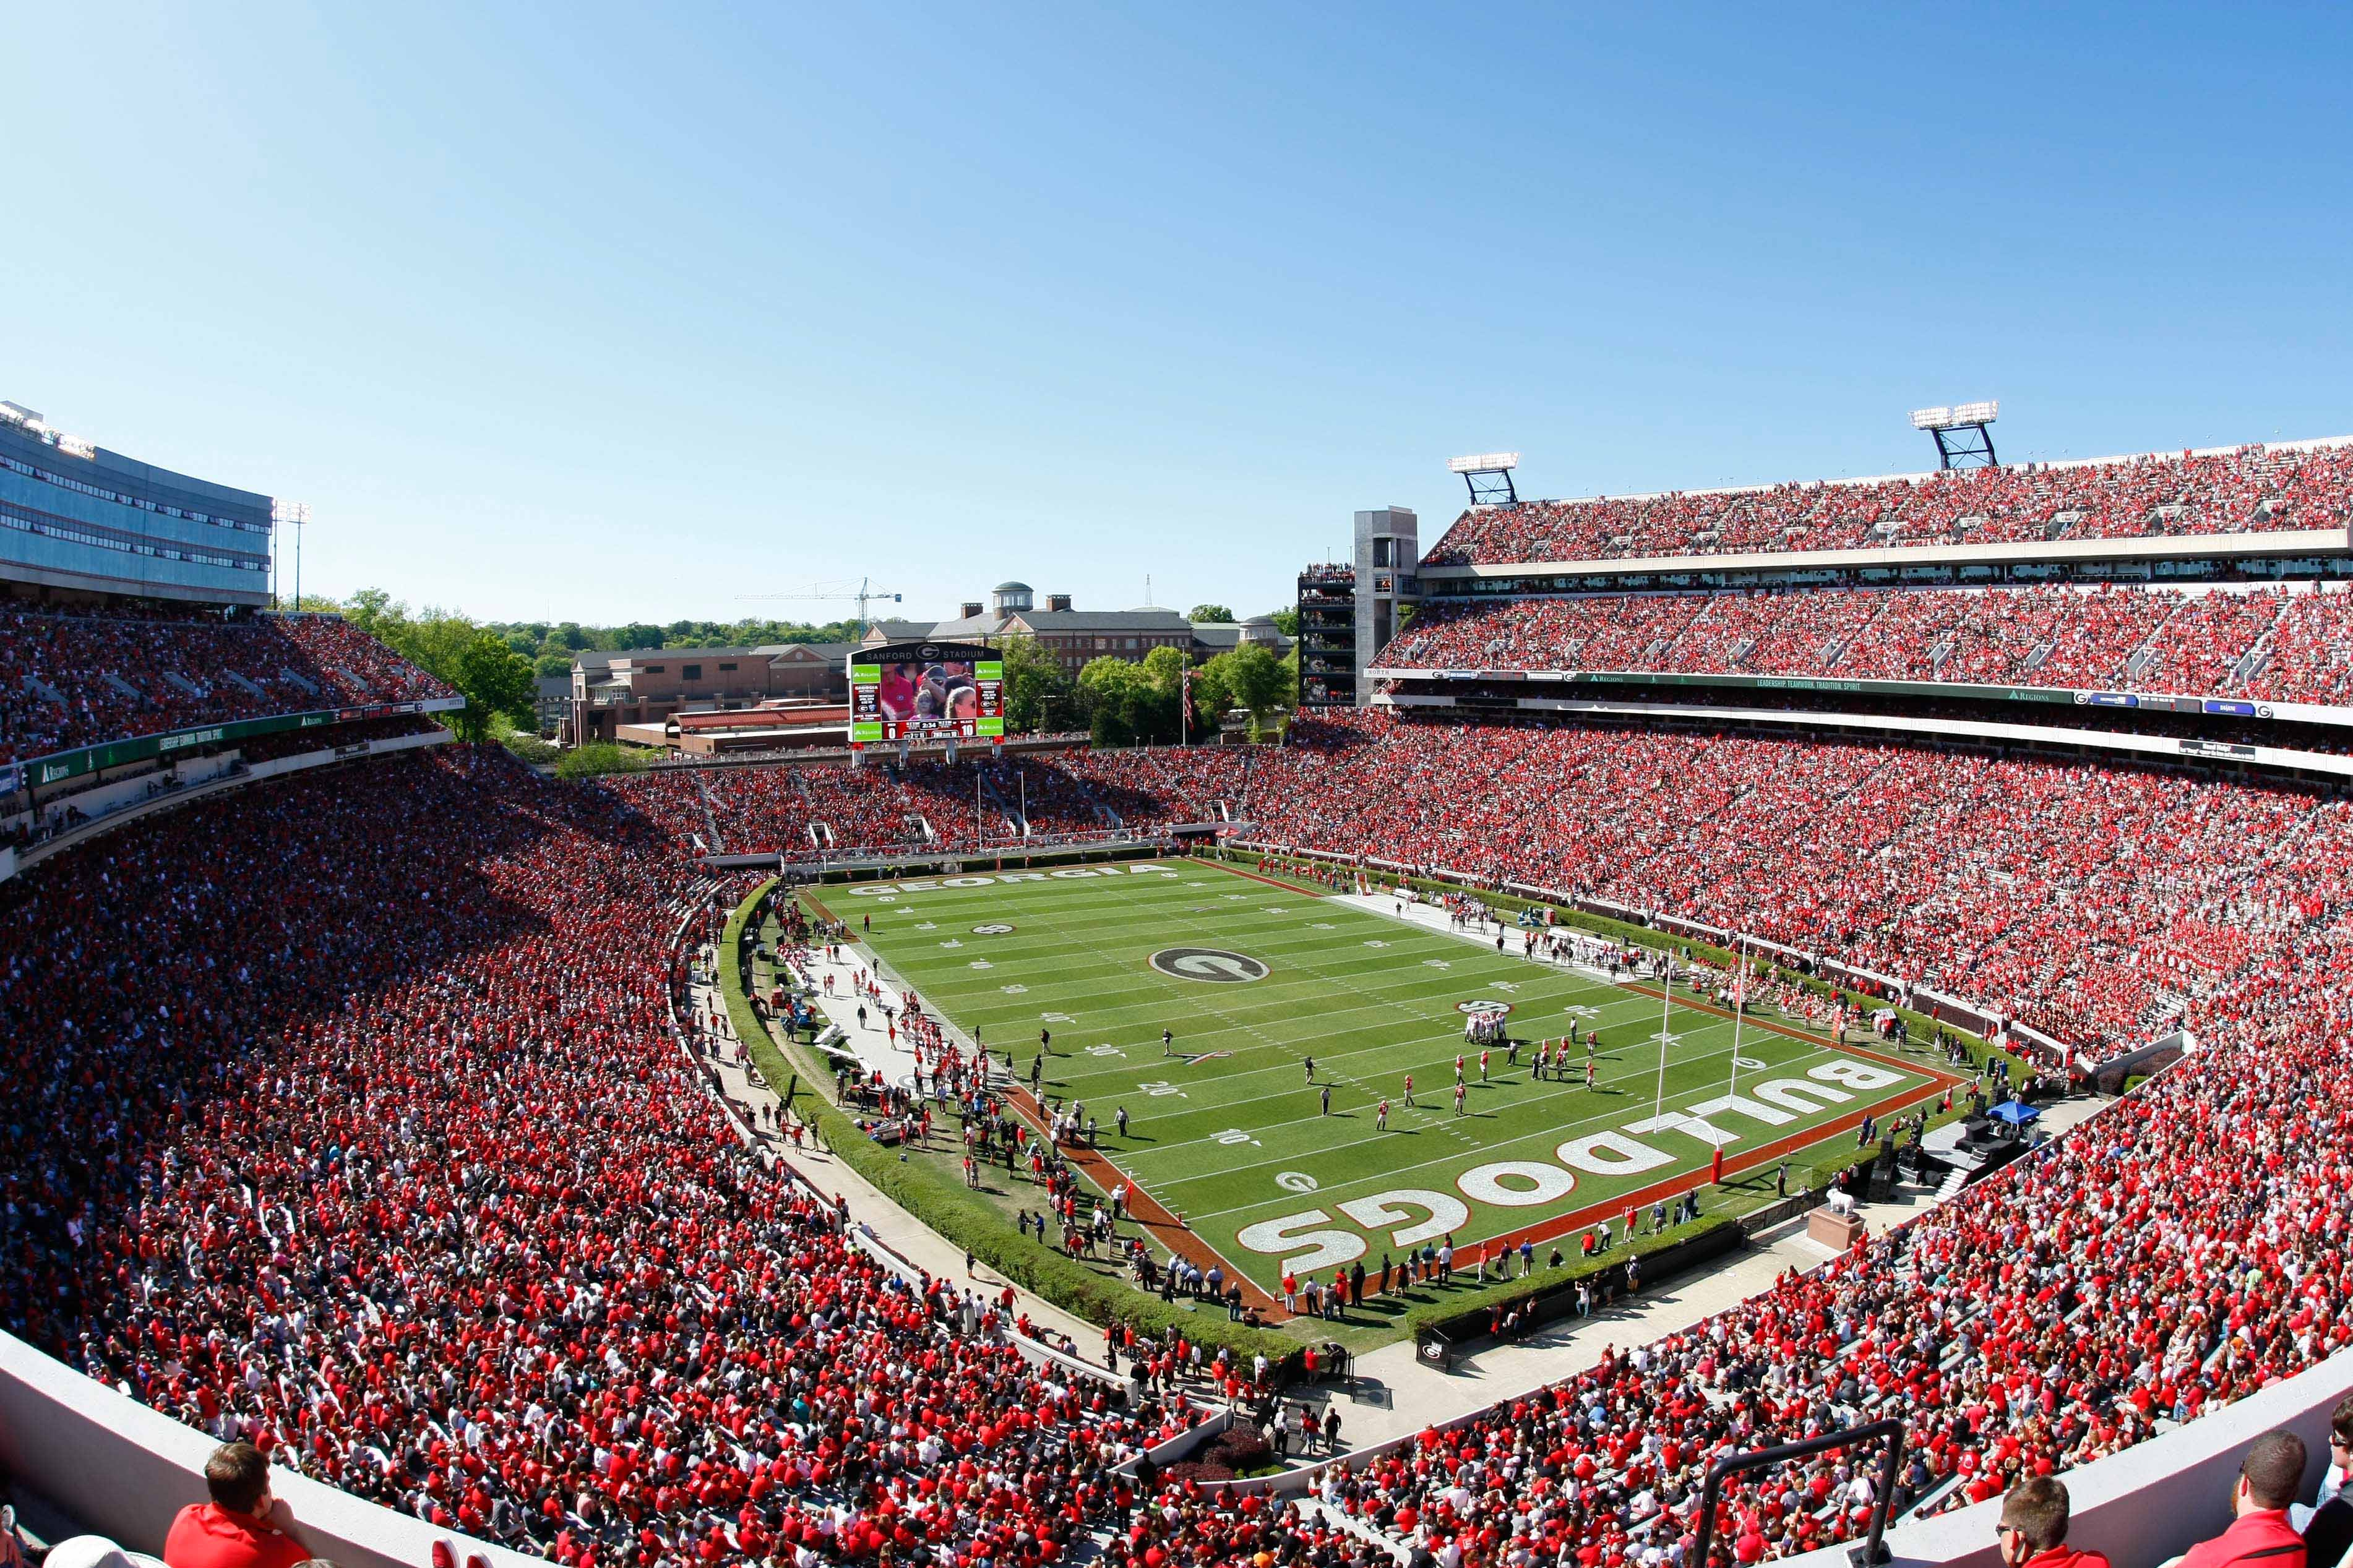
\includegraphics[scale=0.15]{stade.jpeg}
            }
            \only<4>{
              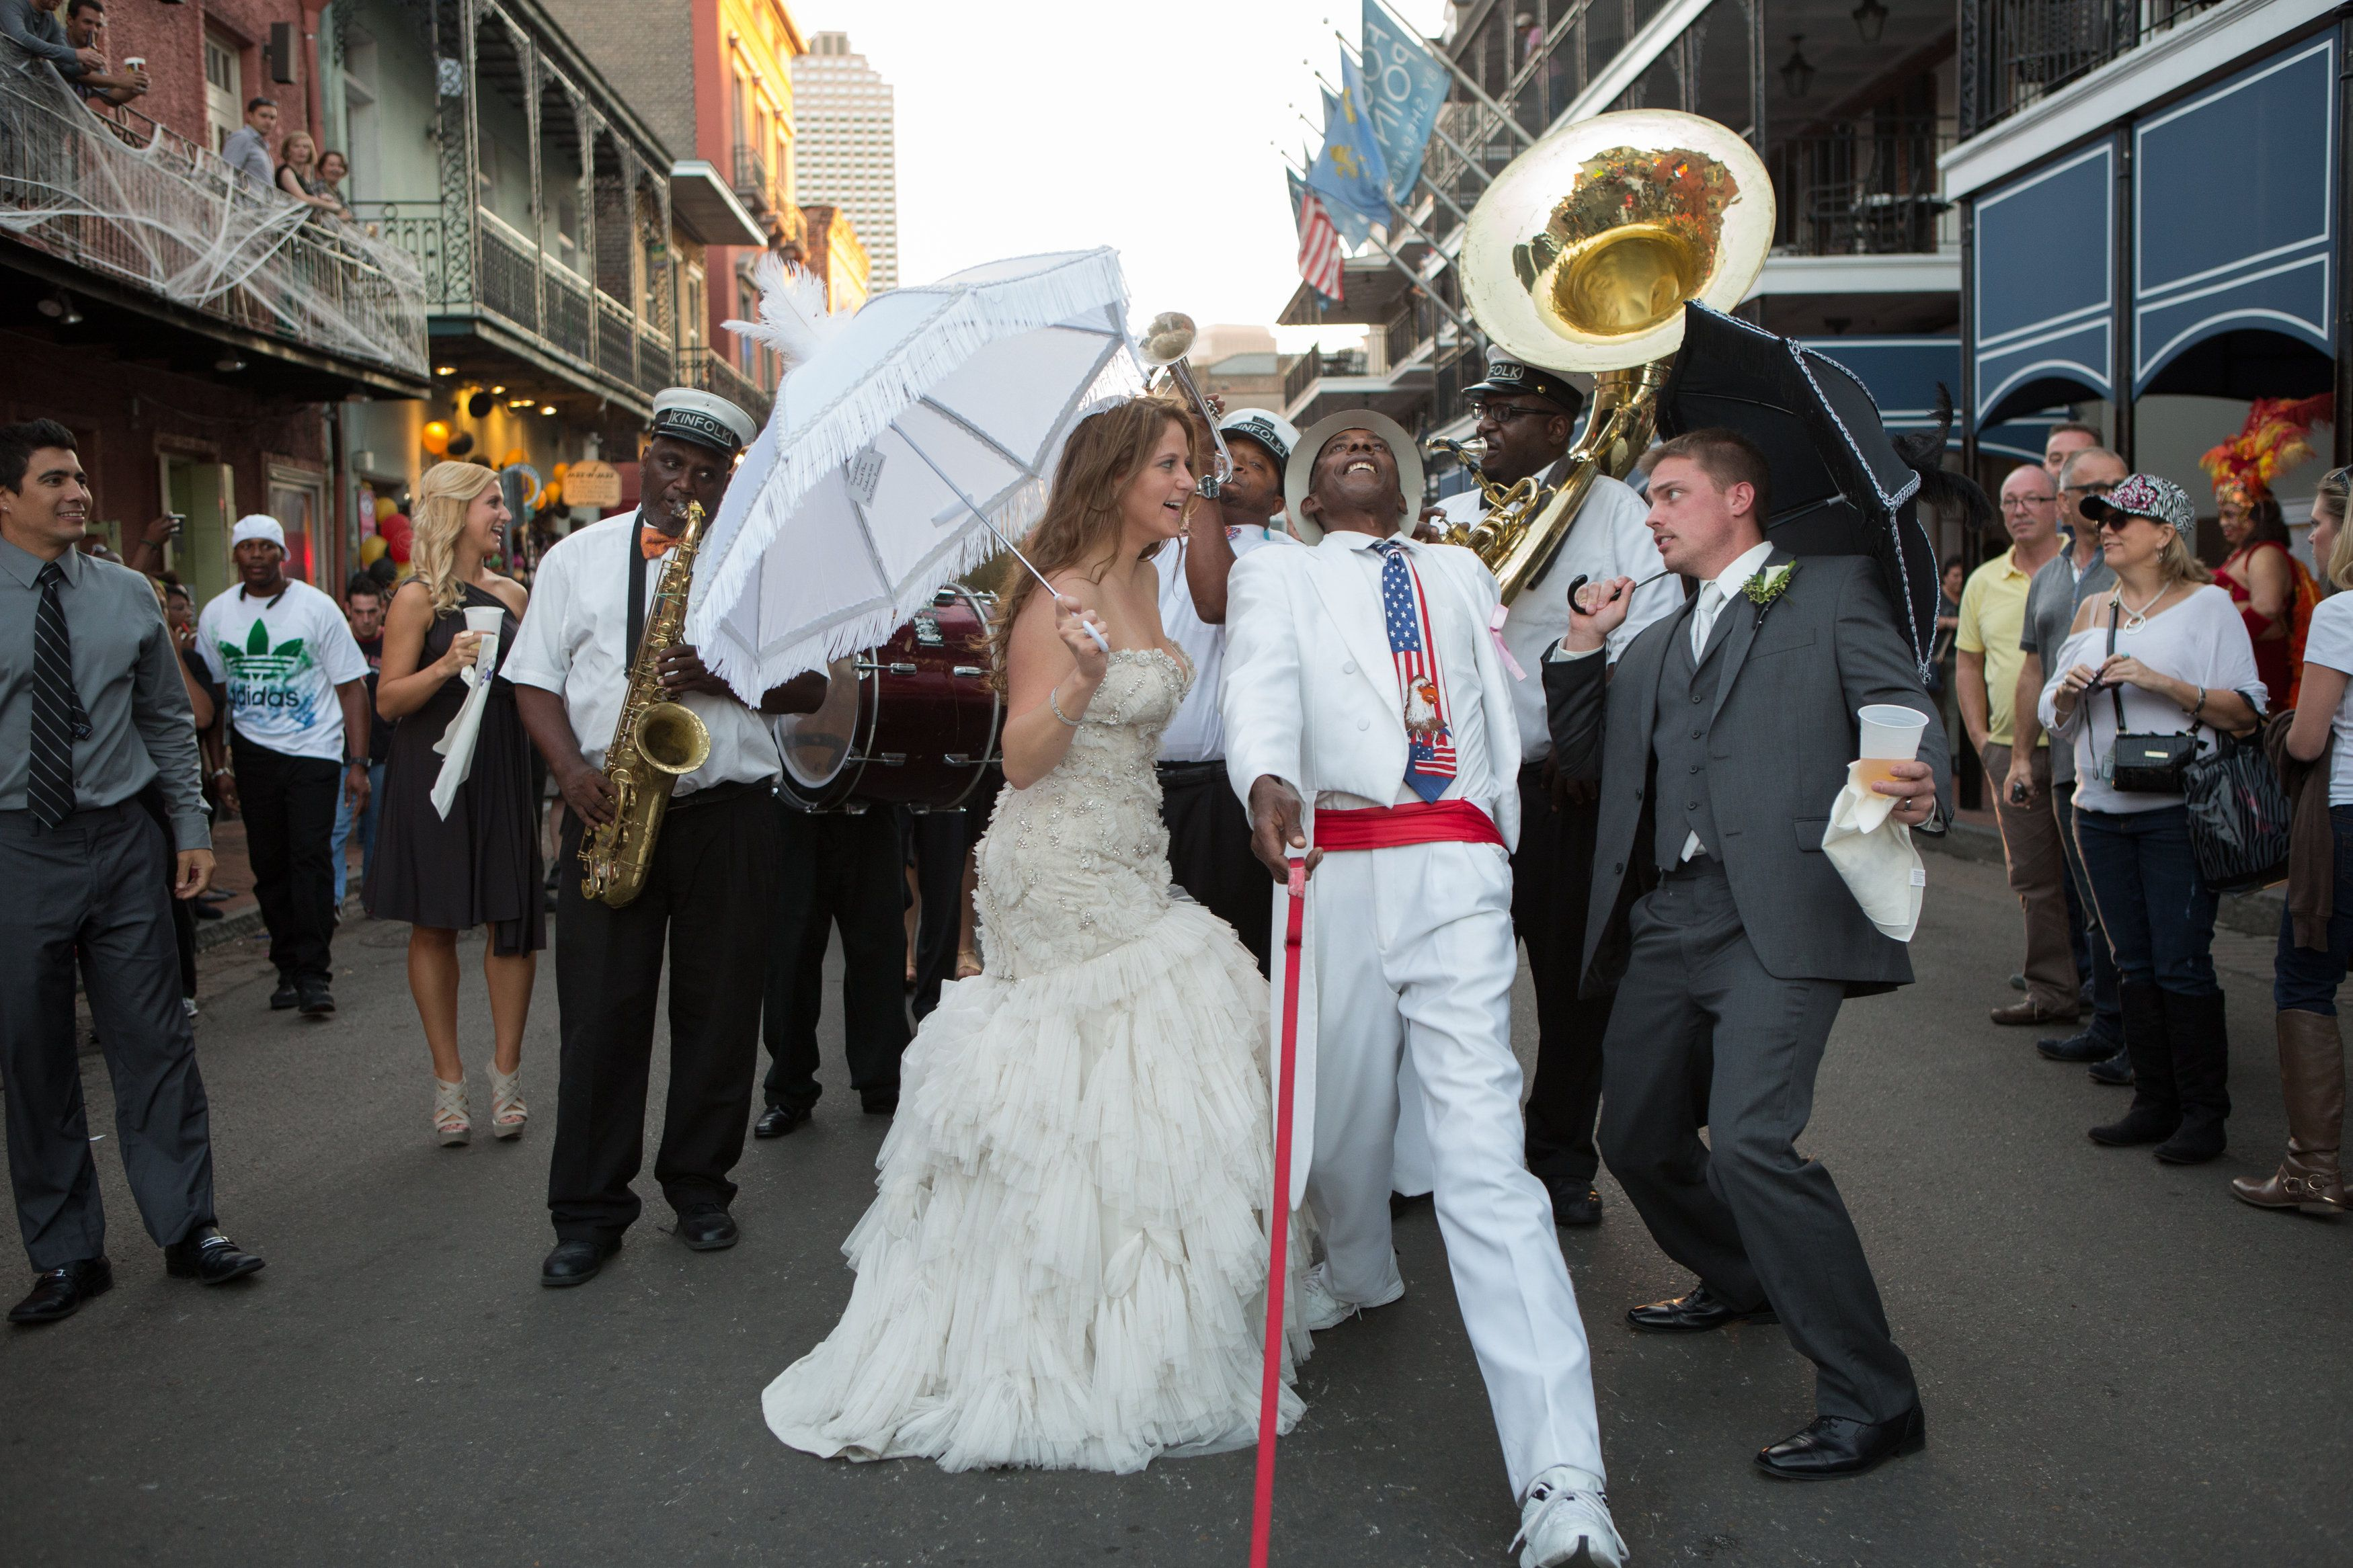
\includegraphics[scale=0.19]{noce.jpg}
            }
            \only<6>{
              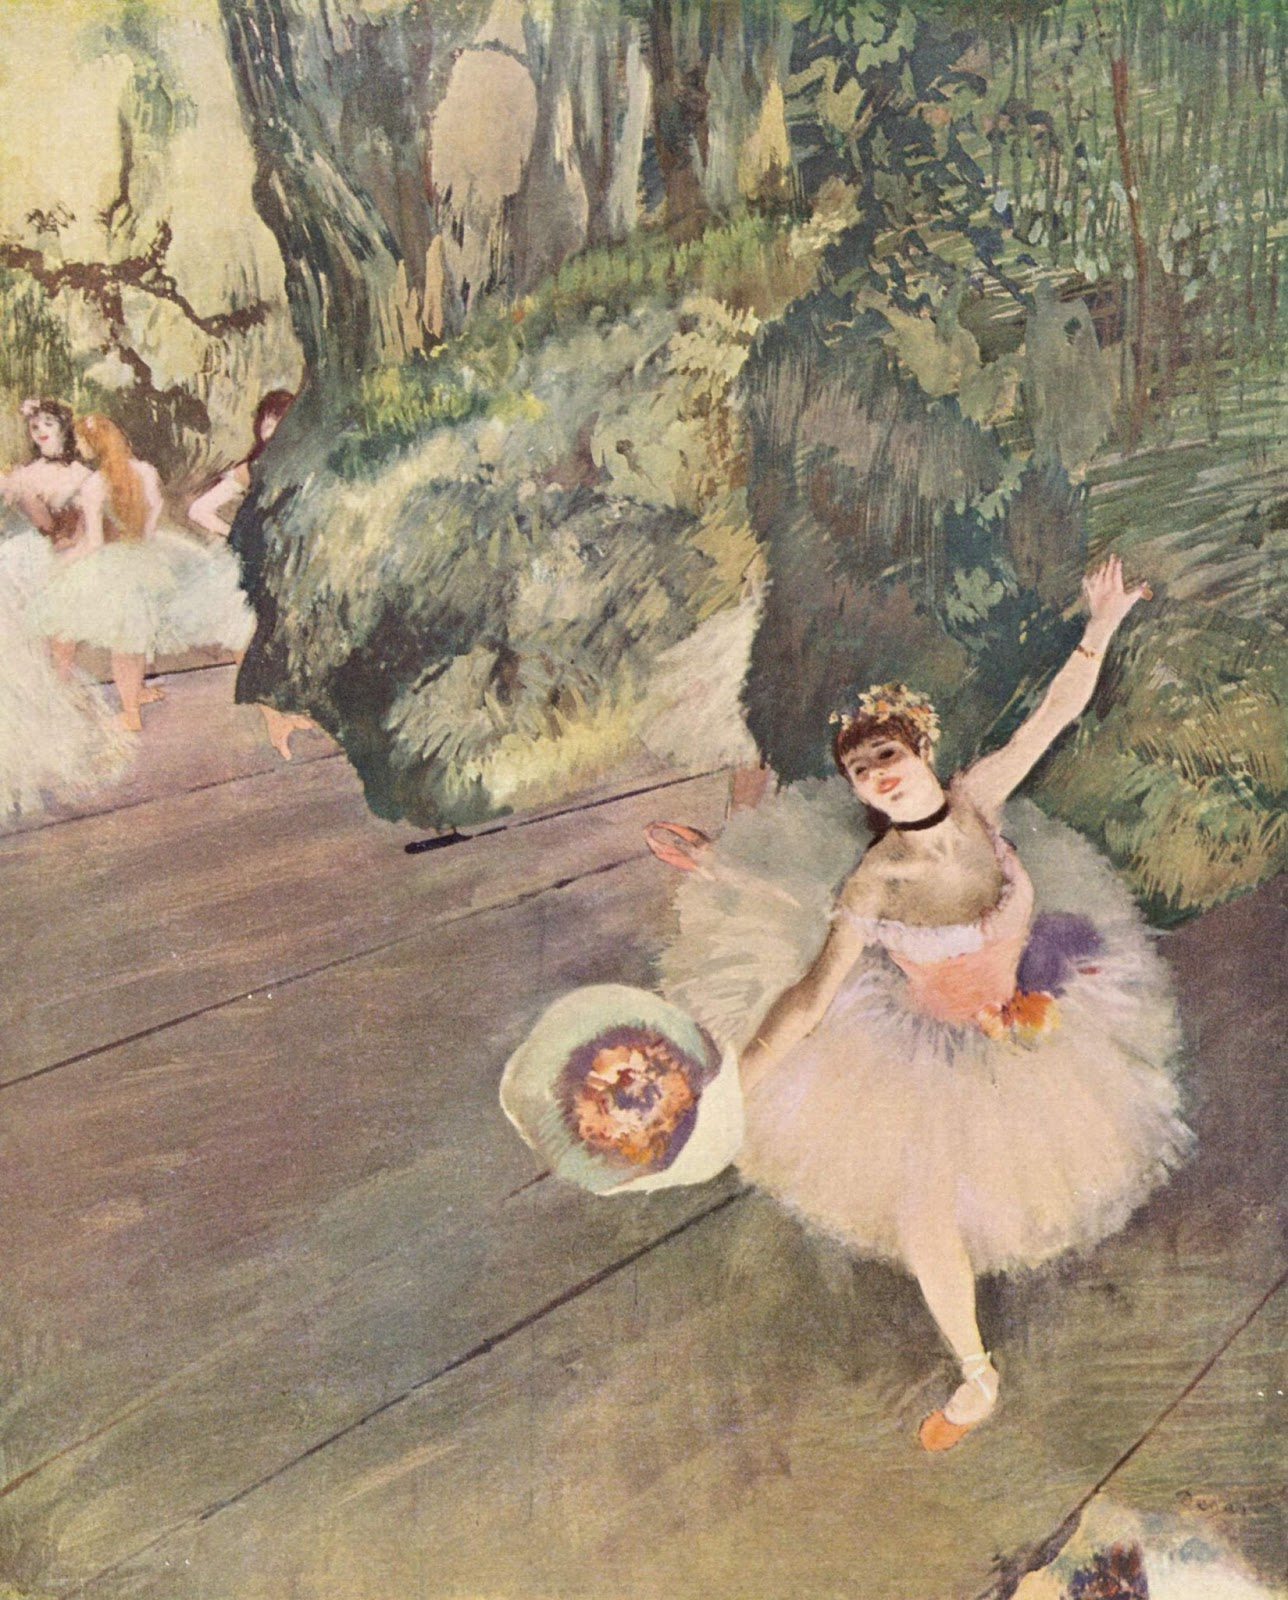
\includegraphics[scale=0.1]{ballet.jpg} \\
              \lexi{L'étoile} par Edgar Degas (1879-1881)
            }
            \only<8>{
              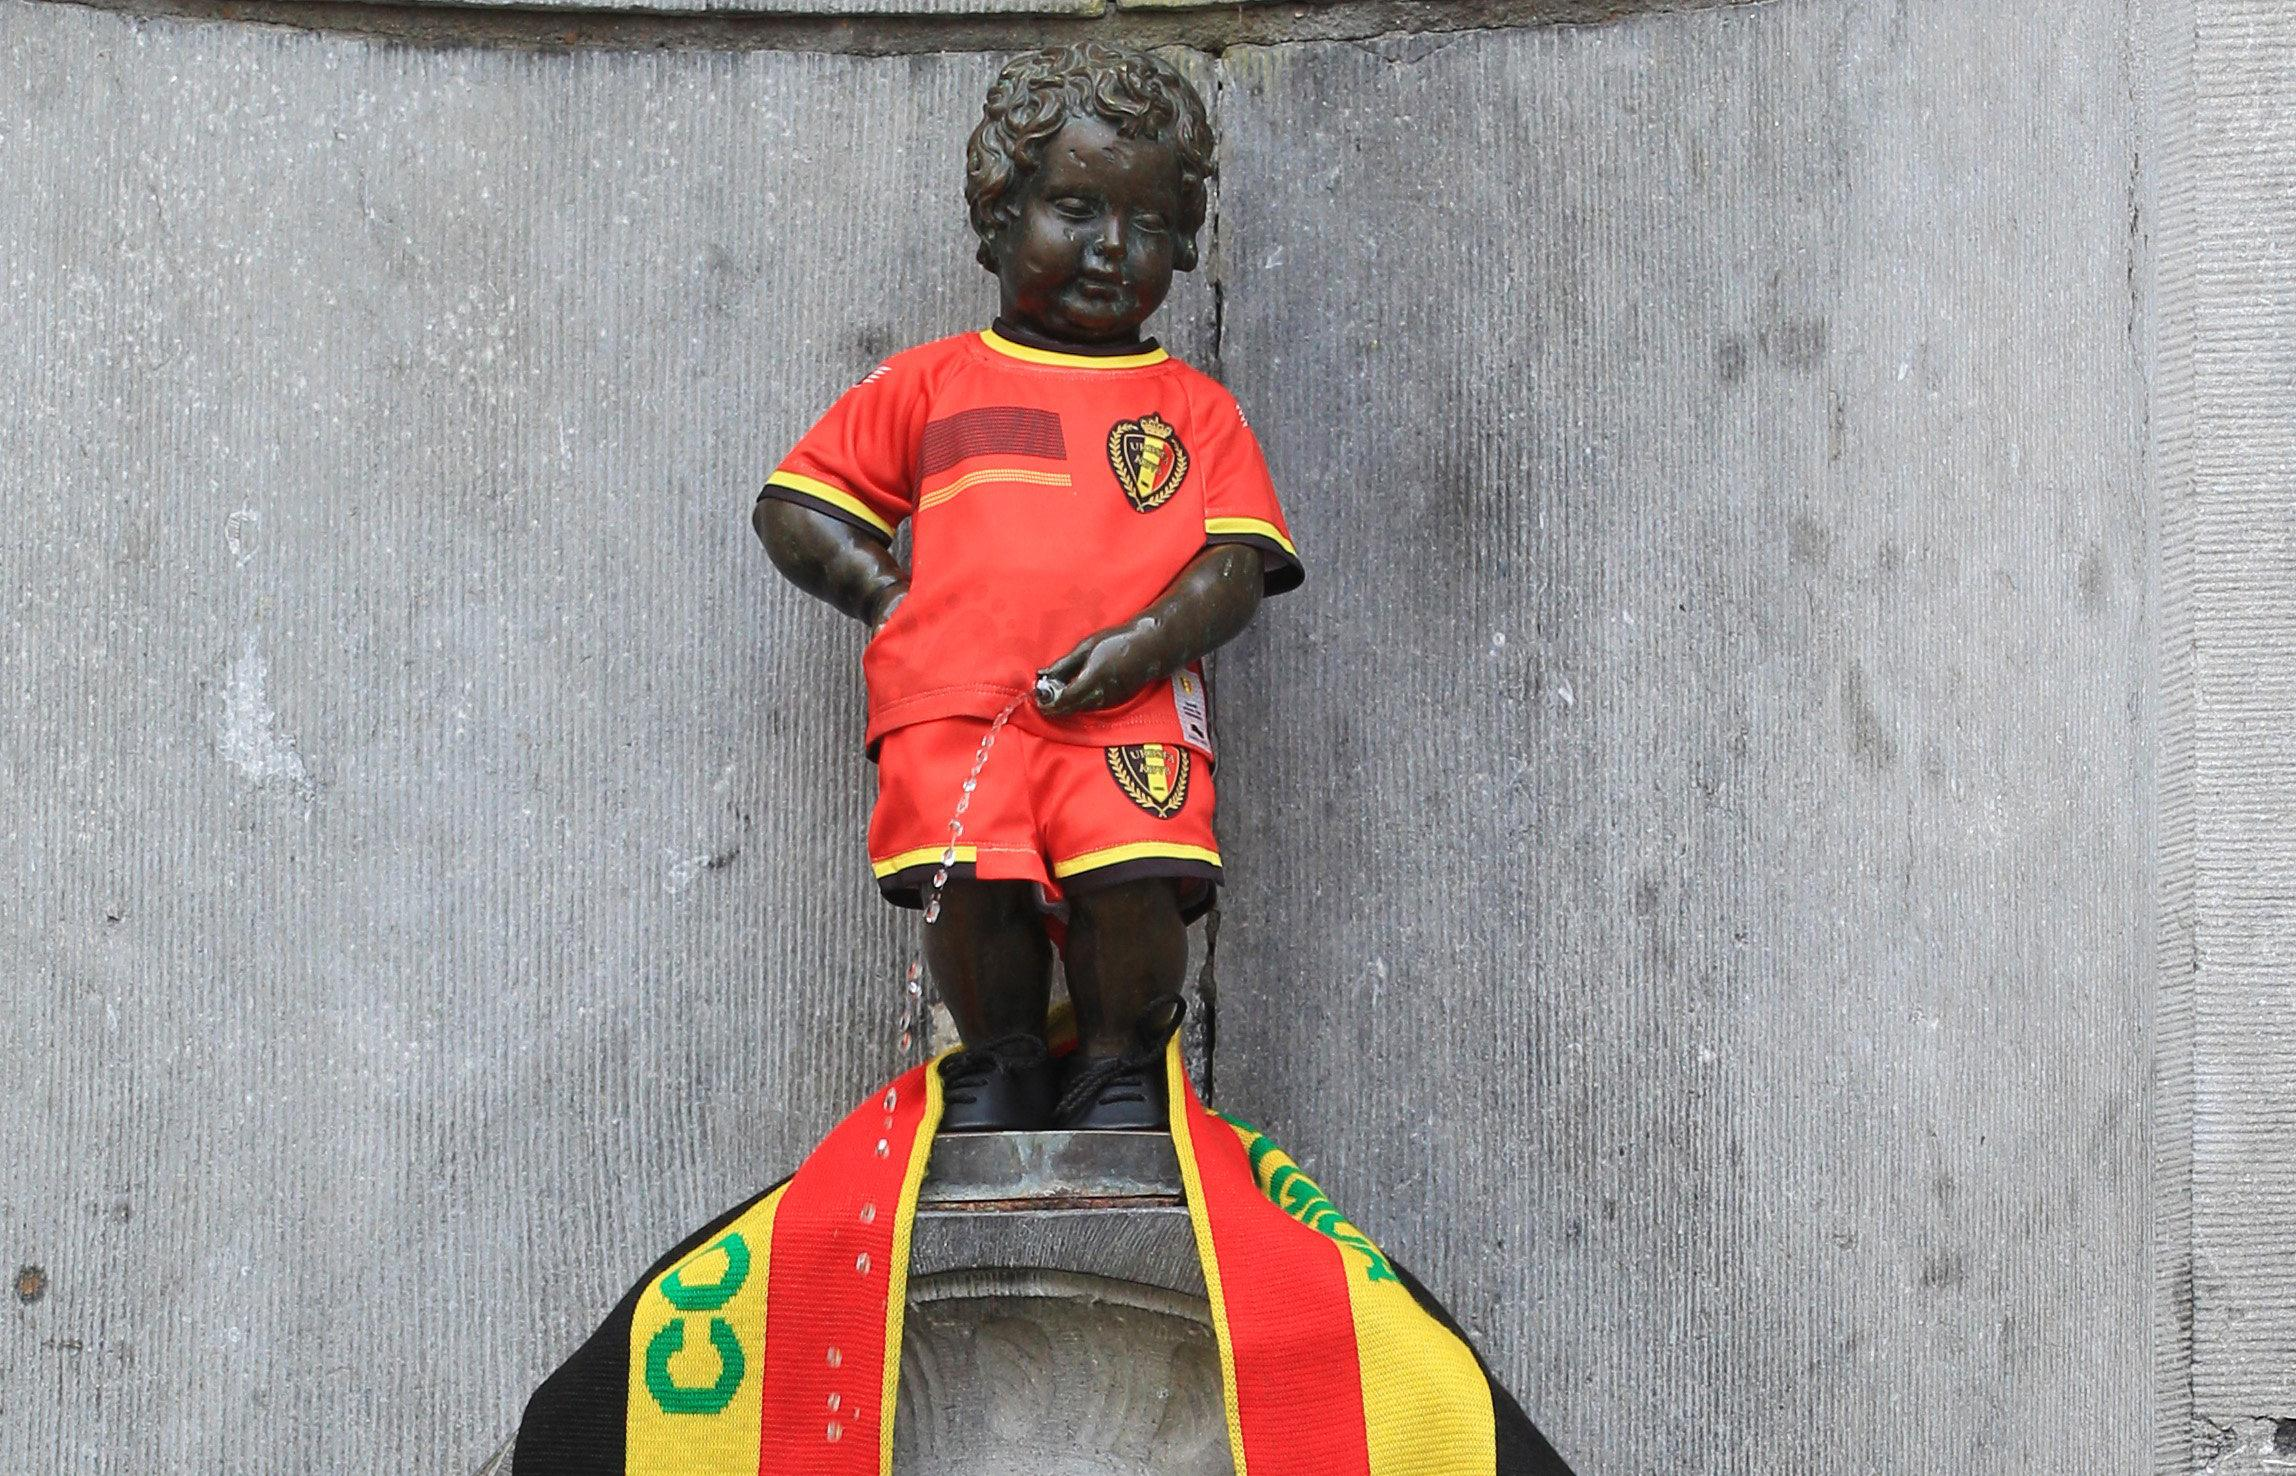
\includegraphics[scale=0.1]{manneken_pis.jpg} \\
              Manneken-Pis à Bruxelles
            }
            \only<10>{
              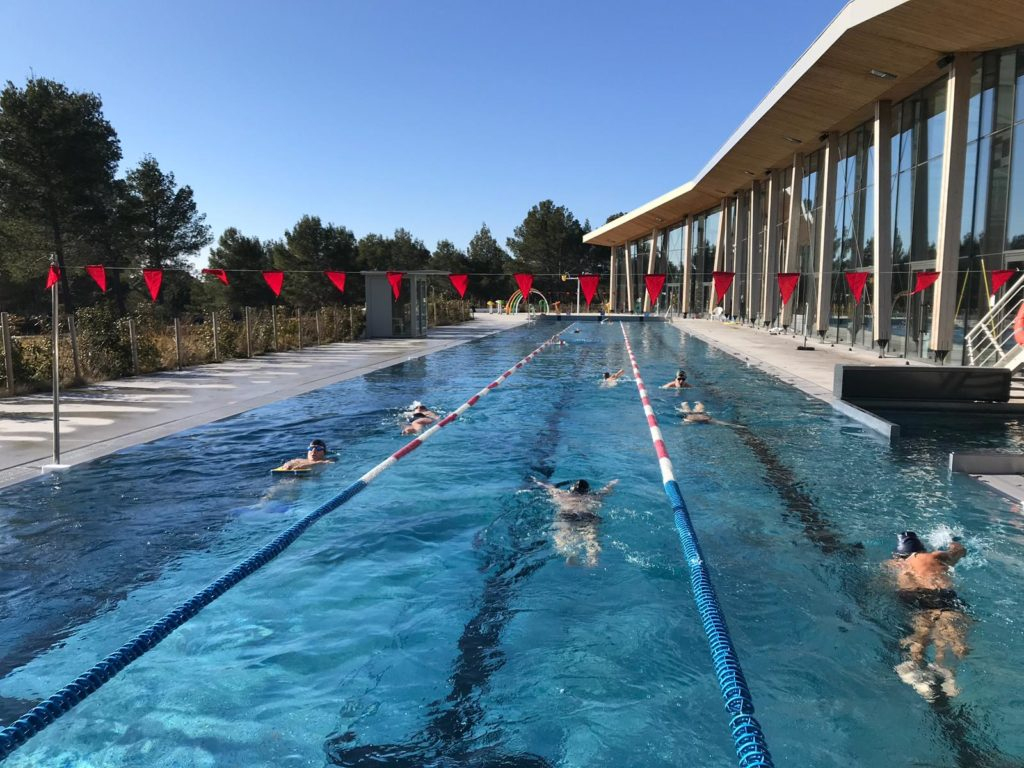
\includegraphics[scale=0.22]{piscine.jpeg}
            }
            \only<12>{
              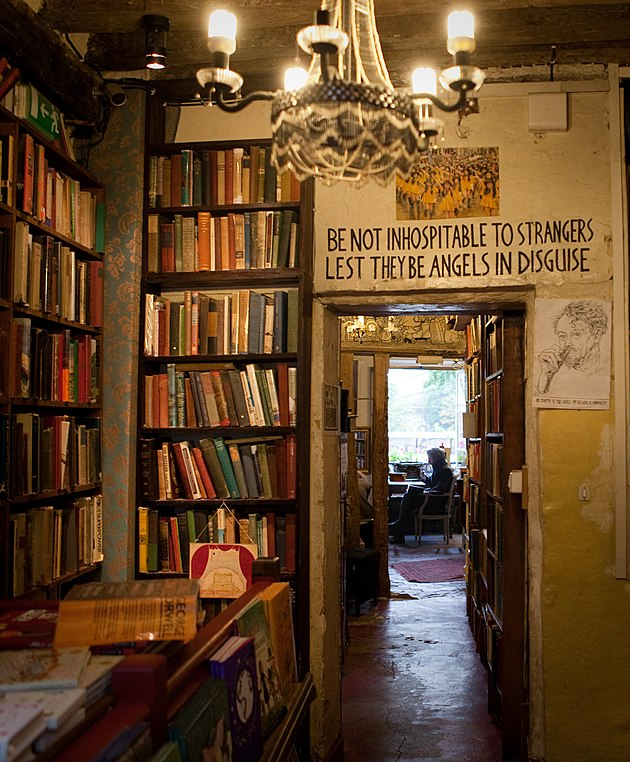
\includegraphics[scale=0.23]{librairie.jpg} \\
              Shakespeare and Company à Paris
            }
          \end{center}
        \end{minipage}
    \end{columns}
  \end{frame}

  \begin{frame}{Vos endroits préférés \gloss{Your favorite places}}
    Avec un partenaire, échangez vos endroits préférés pour les activités suivantes. \\
    \tinygloss{With a partner, share with each other your favorite places to do the following activities.}
    \begin{columns}
      \column{0.5\textwidth}
        \begin{description}
          \item[] \textbf{Modèle:}
          \item[] \emph{pour dîner?}
          \item[E1:] J'aime dîner chez ma mère. Et toi?
          \item[] \tinygloss{I like to eat dinner at my mother's place. And you?}
          \item[E2:] Moi, j'aime dîner au restaurant.
          \item[] \tinygloss{Me, I like to eat diner at the restaurant.}
        \end{description}
      \column{0.5\textwidth}
        \begin{enumerate}
          \item pour dîner?
          \item pour travailler?
          \item pour voir un film?
          \item pour discuter avec des amis?
          \item pour pratiquer un sport?
          \item pour écouter de la musique?
        \end{enumerate}
    \end{columns}
  \end{frame}

  \begin{frame}{Les impératifs \gloss{Imperatives}}
    Quelle est la bonne conjugaison à l'impératif? \\
    \tinygloss{What is the correct conjugation in the imperative?}
    \begin{enumerate}
      \item \underline{\uncover<2->{Mange}} (manger, informal) avec ton frère.
      \item \underline{\uncover<3->{Nageons}} (nager, suggestion) à la piscine.
      \item \underline{\uncover<4->{Jouez}} (jouer, multiple people) au basket.
      \item N'\underline{\uncover<5->{oubliez}} (oublier, formal) pas que je travaille ce soir.
      \item \underline{\uncover<6->{Cherche}} (chercher, informal) le chien chez ta tante.
    \end{enumerate}
  \end{frame}

  \begin{frame}{Des situations \gloss{Some situations}}
    Avec un partenaire, donnez des exemples des impératifs qu'on entendrait dans chaque situation.
    Sur le tableau, écrivez un de vos exemples. \\
    \tinygloss{With a partner, give some examples of some imperatives that you would hear in each situation.
    On the board, write one of your examples.}
    \begin{columns}
      \column{0.5\textwidth}
        \begin{description}
          \item[] \textbf{Modèle:}
          \item[] \emph{une mère à son enfant}
          \item[$\to$] Fais tes devoirs.
          \item[] \tinygloss{Do your homework.}
        \end{description}
      \column{0.5\textwidth}
        \begin{enumerate}
          \item un professeur aux étudiants
          \item une étudiante à un/e ami/e
          \item un étudiant au professeur
          \item un étudiant à son copain
          \item un coach à ses joueurs
          \item une musicienne au public
          \item un président à un sénateur
        \end{enumerate}
    \end{columns}
  \end{frame}

  \begin{frame}{}
    \begin{center}
      \Large Questions?
    \end{center}
  \end{frame}
\end{document}
